\chapter{Введение. Задача Person Re-Identification (Re-Id)}
\label{ch:введение}

\newcommand{\reid}{Person Re-Identification}
\newcommand{\bbox}{bounding box}

\section{Задача Person Re-Identification}

\reid\ $-$ задача компьютерного зрения, цель которой состоит в том, чтобы распознавать людей на видео или отдельных кадрах с различных камер видеонаблюдения и в разных локациях. Она включает в себя обнаружение и отслеживание человека на видео и дальнейшее использование таких признаков, как внешний вид, телосложение и одежда, для сопоставления его личности на разных кадрах. Итоговая цель $-$ возможность обнаружить и идентифицировать одного и того же человека на различных непересекающихся видах с камер, расположенных в различных местах города или предприятия. 

Кроме идентификации людей, данная постановка задачи применима также, например, для систем мониторинга автомобилей на дорогах, для наблюдения за наличием товаров на полках магазинов, для отслеживания местоположения животных в заповедниках по данным с фотоловушек, а также для поиска потерявшихся домашних животных. Однако наиболее часто целевыми объектами являются люди, поэтому по умолчанию говорят именно о задаче идентификации людей, что зафиксировано и в традиционном названии $-$ \reid.

На \hyperref[fig:prid_2022_images_example]{Рисунке \ref*{fig:prid_2022_images_example}} можно увидеть пример изображений, которые нужно обрабатывать. Для каждого человека имеется некоторое количество кадров с разных камер. На примере каждая строка соответствует одному человеку, первые три кадра в строке получены с одной камеры, а последние три $-$ с другой. Задача состоит в том, чтобы идентифицировать все эти кадры как изображения одного и того же объекта, то есть одного и того же человека.

\begin{figure}[ht]
    \centering
    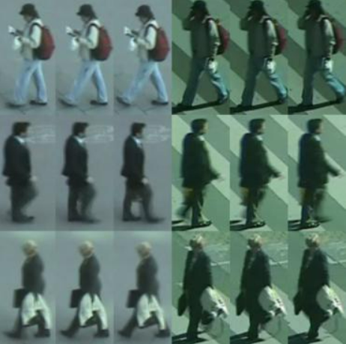
\includegraphics[width=0.5\textwidth]{images/reid_problem/prid2011.png}
    \caption{Пример изображений из набора PRID2011 \cite{hirzer2011person}}
    \label{fig:prid_2022_images_example}
\end{figure}

\section{Общая схема решения}

Общая схема работы над решением задачи \reid\ проиллюстрирована на \hyperref[fig:general_pipeline]{Рисунке \ref*{fig:general_pipeline}}. Во-первых, собираются данные с камер видеонаблюдения $-$ это исходные видео. Далее на каждом кадре размечаются \textit{\bbox}-ы $-$ прямоугольные участки изображения, в которых находятся целевые объекты. Далее каждому \bbox-у присваивается метка $-$ уникальный идентификатор человека, изображенного на кадре внутри данного \bbox-а. Теперь, когда получена разметка, следует этап обучения модели компьютерного зрения для идентификации человека по изображению. А именно, обучается нейросеть, которая строит векторные представления поступающих на вход изображений. Получаемые таким образом векторные представления используются на последнем этапе работы системы $-$ поиске соответствующего объекта в базе данных на основе близости векторных представлений.

\begin{figure}[ht]
    \centering
    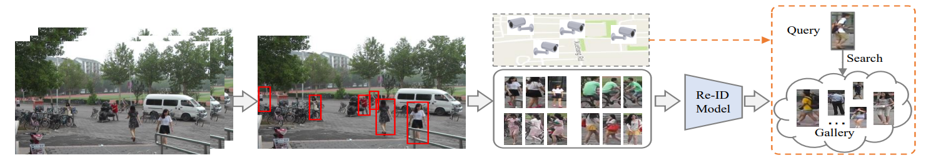
\includegraphics[width=\textwidth]{images/reid_problem/general_pipeline.png}
    \caption{Общая схема решения задачи Re-Id \cite{ye2021deep}}
    \label{fig:general_pipeline}
\end{figure}

\section{Математическая постановка задачи}

В рамках общей прикладной задачи можно выделить формальную математическую составляющую. Согласно ей, рассматриваются два множества изображений $-$ $Query$ и $Search$ (от английских названий \textit{query space} и \textit{search space} $-$ пространство запросов и пространство поиска). $Search$ представляет собой базу данных, в которой хранятся \textit{размеченные}, то есть известные изображения. Таким образом, для каждого изображения $x_j \in Search$ известна метка идентификации человека $y_j$ $-$ уникальный идентификатор, например, число в диапазоне от $1$ до $N$, где $N$ $-$ количество различных людей в базе. При этом $N \leqslant |Search|$ $-$ для каждого человека в базе может быть представлено одно или несколько изображений.

Каждый объект $q_i \in Query$ представляет собой изображение-запрос, то есть фотографию человека, личность которого неизвестна, и которую требуется установить. Для каждого $q_i$ в базе данных есть целевое множество $T_i \in Search$ $-$ множество тех картинок в базе, на которых запечатлен тот же человек. Задача состоит в том, чтобы для каждого $q_i$ выдать \textit{ранжированный список} из элементов базы, то есть перестановку $r_i \in S_{|Search|}$ из индексов в диапазоне $\overline{1, |Search|}$. Здесь $S_n$ $-$ группа всех перестановок элементов множества $\overline{1, n}$ $-$ натуральных чисел от 1 до $n$ включительно. Цель состоит в том, чтобы целевые изображения занимали позиции в начале данного списка, а изображения других людей $-$ после них. Это соответствует сортировке изображений по степени уверенности в том, что на них представлен тот же человек, что и в запросе. На \hyperref[fig:ranked_list]{Рисунке \ref*{fig:ranked_list}} представлен пример ранжированного списка. Зеленым отмечены целевые изображения, красным $-$ изображения других людей. 

Далее обсудим метрики качества решения данной задачи $-$ численные выражения соответствия действительности полученных списков.

\begin{figure}[ht]
    \centering
    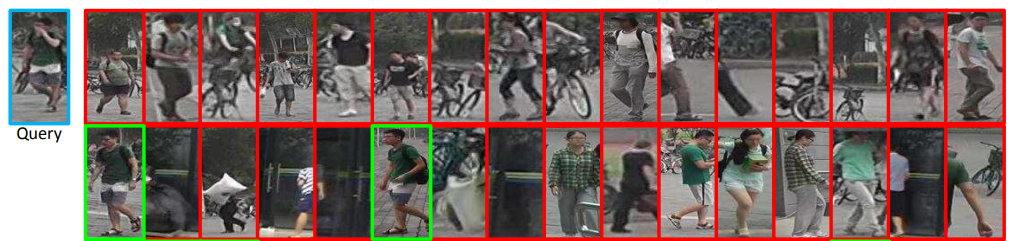
\includegraphics[width=\textwidth]{images/reid_problem/task_ranked_list.png}
    \caption{Пример ранжированного списка для одного запроса \cite{zheng2015scalable}}
    \label{fig:ranked_list}
\end{figure}

\section{Метриики качества}

\subsection{Cumulated Matching Characteristics}

Cumulated Matching Characteristics (CMC) $-$ базовый вариант оценки качества ранжированных списков. Для ее подсчета выбирается пороговое значение $-$ количество элементов от начала списка, которые берутся в рассмотрение. Для заданного порога $k$ значение метрики $CMC @ k$ определяется как доля тех запросов $q_i$, для которых среди первых $k$ элементов ранжированного списка присутствует \textit{хотя бы один} целевой объект $x_j \in T_i$:

\begin{equation}
    CMC @ k = \frac{1}{|Query|} \sum \limits_{i = 1}^{|Query|} \mathbb{I} [r_i[:k] \cap T_i \neq \varnothing].
\end{equation}

Здесь $\mathbb{I}$ $-$ индикаторная функция, $r_i[:k]$ $-$ первые $k$ элементов ранжированного списка $r_i$. Данная метрика качества в первую очередь применима в тех случаях, когда для каждого запроса в базе присутствует только один целевой объект, или, например, когда $k = 1$ $-$ при рассмотрении первого элемента списка. В случае же, если целевых объектов несколько, то при подсчете по данной формуле не учитывается порядок элементов в рассматриваемой части списка. Поэтому значение метрики будет одинаковым, независимо от того, расположен целевой объект на первых позициях или ближе к концу участка $r_i[:k]$, хотя с практической точки зрения первый вариант является более предпочтительным. Для того, чтобы преодолеть эту проблему, была введена еще одна метрика качества $-$ Mean Average Precision.

\subsection{Mean Average Precision}

Данная метрика, сокращенно $mAP$, позволяет учесть в том числе и положение целевых объектов в рассматриваемом участке ранжированного списка \cite{zheng2015scalable}. Эта метрика строится на основе стандартных метрик бинарной классификации $precision$ и $recall$: вычислется среднее значение площади под кривой Precision-Recall для всех целевых объектов. Формально, для запроса $q_i$ и каждого порога $k$ вычисляется значение

\begin{equation}
    P_i(k) = \frac{1}{k} \sum \limits_{j = 1}^{k} \mathbb I [r_i[j] \in T_i].
\end{equation}

Далее,

\begin{equation}
    AP_i = \frac{1}{|T_i|} \sum \limits_{k = 1}^{|Search|} P_i(k).
\end{equation}

И, наконец, 

\begin{equation}
    mAP = \frac{1}{|Query|} \sum \limits_{i = 1}^{|Query|} AP_i.
\end{equation}

Также применяется вариант этой метрики $-$ $mAP@k$, получаемый рассмотрением в $AP_i$ только первых $k$ элементов списка $r_i$. 

На \hyperref[fig:cmc_map]{Рисунке \ref*{fig:cmc_map}} на примере проведено сравнение CMC и mAP. Для всех трех списков значение CMC будет равно $1$, однако mAP позволяет отразить, что второй список предпочтительнее третьего.

\begin{figure}[ht]
    \centering
    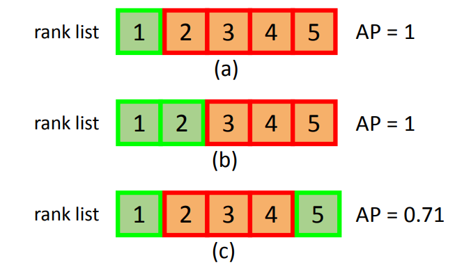
\includegraphics[width=0.5\textwidth]{images/reid_problem/metrics_example.png}
    \caption{Сравнение CMC и mAP. Для всех трех списков CMC = $1$, в то время как AP равны 1, 1 и 0.71 \cite{zheng2015scalable}}
    \label{fig:cmc_map}
\end{figure}

\section{Датасеты}

Для построения качественных систем решения задачи \reid\ существуют различные публичные датасеты, которые предоставляют большие наборы размеченных данных для обучения ML-моделей. Также они служат \textit{бенчмарками} $-$ позволяют сравнивать качество моделей на тестовой части датасета. Первые датасеты для данной задачи существуют с 2007 года. Со временем происходило увеличение датасетов $-$ как по количеству изображений, так и по количеству представленных на них людей. 

В \hyperref[tab:datasets]{Таблице \ref*{tab:datasets}} приведены характеристики основных датасетов для задачи Re-Id. Со временем в датасеты стали включаться не только размеченные вручную \bbox-ы, но и полученные автоматически с помощью ML-моделей детекции. Также некоторые датасеты включают наборы изображений-дистракторов $-$ тех кадров, которые содержат лишь фон. Включение таких изображений позволяет добиваться от системы более достоверных предсказаний, учитывающих возможность ложных срабатываний детектора людей, предоставляющего \bbox-ы. Также важно, чтобы система могла работать с изображениями разного качества, поэтому в современные датасеты включают кадры как низкого, так и высокого разрешения.

\begin{table}[]
    \centering
    \caption{Сравнение различных датасетов. Год $-$ год публикации, \#ID $-$ количество представленных людей, \#кадров $-$ общее количество изображений, \#камер $-$ количество разных камер, Размет. $-$ ручная, автоматическая или смешанная разметка \bbox-ов, Разреш. $-$ фиксированное или различное разрешение, Метрика $-$ только CMC или CMC и mAP (С \& M) \cite{ye2021deep}}
    \begin{tabular}{|l|l|l|l|l|l|l|l|}
        \hline
        \multicolumn{1}{|l|}{Датасет} & \multicolumn{1}{l|}{Год} & \multicolumn{1}{l|}{\#ID} & \multicolumn{1}{l|}{\#кадров} & \multicolumn{1}{l|}{\#камер} & \multicolumn{1}{l|}{Размет.} &
        \multicolumn{1}{l|}{Разреш.} & \multicolumn{1}{l|}{Метрика} \\ \hline
        VIPeR & 2007 & 632 & 1 264 & 2 & ручная & фикс & CMC \\ \hline
        PRID2011 & 2011 & 200 & 1 134 & 2 & ручная & фикс & CMC \\ \hline
        CUHK03 & 2014 & 1 467 & 13 164 & 2 & ручная & разн & CMC \\ \hline
        Market-1501 & 2015 & 1 501 & 32 668 & 6 & смеш & фикс & C\&M \\ \hline
        DukeMTMC & 2017 & 1 404 & 36 411 & 8 & смеш & фикс & С\&M \\ \hline
        MSMT17 & 2018 & 4 101 & 126 441 & 15 & авто & разн & С\&M \\ \hline
    \end{tabular}
    \label{tab:datasets}
\end{table}

На  \hyperref[fig:market_example]{Рисунке \ref*{fig:market_example}} приведены примеры изображений из датасета Market-1501, которые включает в себя виды с различных камер, а также изображения-дистракторы.

\begin{figure}[ht]
    \centering
    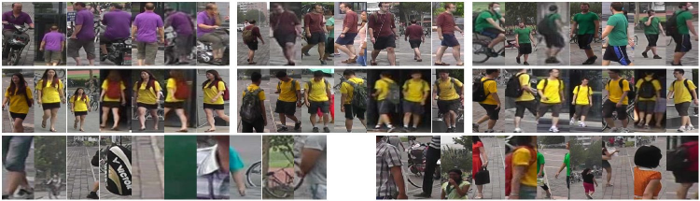
\includegraphics{images/closed_world/market_example.png}
    \caption{Пример изображений из датасета Market-1501. \cite{zheng2015scalable}}
    \label{fig:market_example}
\end{figure}



\endinput